%!TEX root = ../../presentation.tex

\begin{frame}{The Phase Field Approach to Fracture - General Idea}

\begin{reference}{\refh}{\refv}
Francfort \& Marigo (1998), Miehe et al. (2010), Borden et al. (2012), Miehe \& Sch\"anzel (2014), ...
\end{reference}

\begin{columns} 
\column{.25\textwidth}
  \centering
  \begin{figure}
    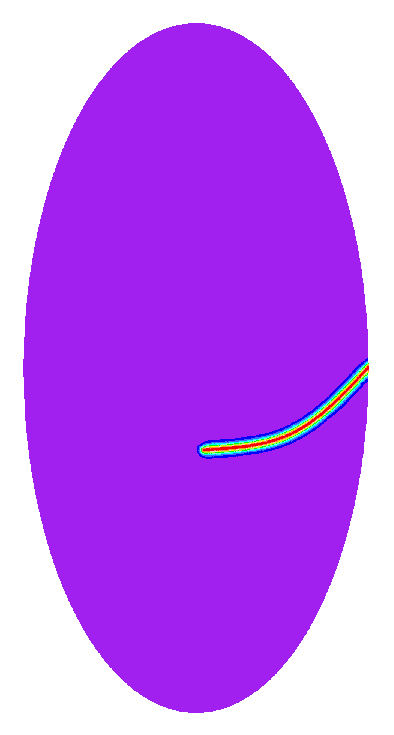
\includegraphics[height=30mm]{\slidedir/f03a}
  \end{figure}
  \vspace{-3mm}{\footnotesize{$l=l_1$}}

\column{.25\textwidth}
  \centering
  \begin{figure}
    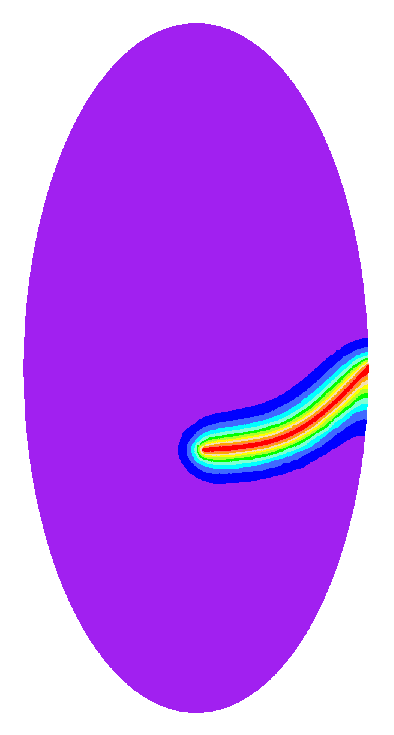
\includegraphics[height=30mm]{\slidedir/f03b}
  \end{figure}
  \vspace{-3mm}{\footnotesize{$l=l_2$}}

\column{.25\textwidth}
  \centering
  \begin{figure}
    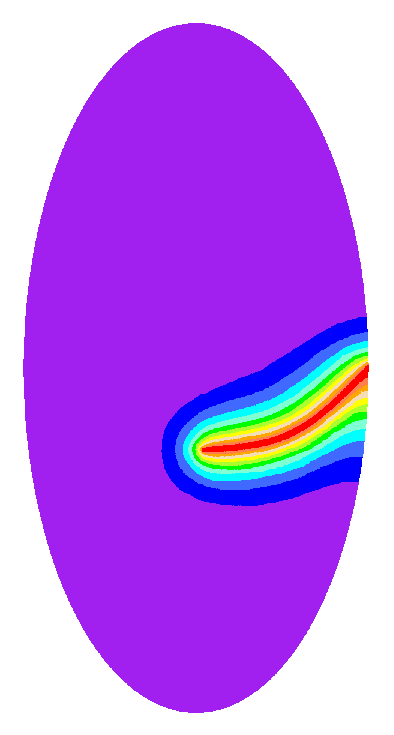
\includegraphics[height=30mm]{\slidedir/f03c}
  \end{figure}
  \vspace{-3mm}{\footnotesize{$l=l_3$}}


\column{.25\textwidth}
  \centering
  \begin{figure}
  {\footnotesize
  \psfrag{d}[c][c]{\scriptsize{\rotatebox{90}{$d$}}}
  \psfrag{l}[c][c]{\scriptsize{\rotatebox{90}{$2l$}}}
  \psfrag{1}[c][c]{\scriptsize{\rotatebox{90}{$1$}}}
  \psfrag{x}[c][c]{\scriptsize{\rotatebox{90}{$x$}}}
  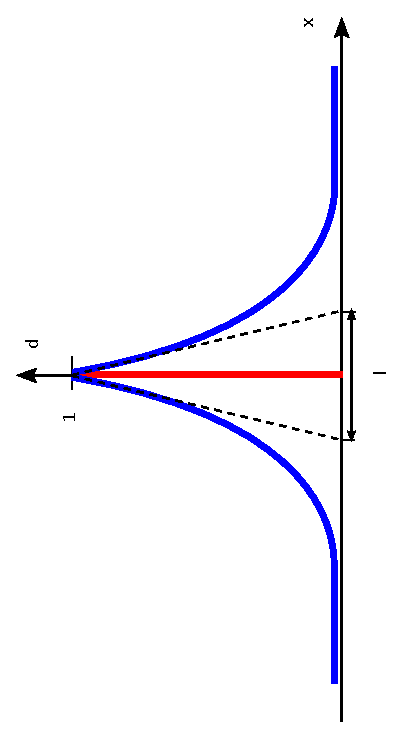
\includegraphics[height=30mm]{\slidedir/f03d}}
  \end{figure}
  \vspace{-3mm}{\footnotesize{solution of d}}
\end{columns}

\bigskip
\bigskip
\bigskip

Phase field models approximate the sharp failure surface $\Gamma$ by a diffusive crack topology described by 
\begin{equation*}
  d(x)=e^{-|x|/l} \quad \text{being the solution of} \quad d(x)-l^2d''(x)=0 \quad \text{in} \quad \body
\end{equation*}

\smallskip

The fracture energy can then be approximated as
\begin{equation*}
  W_c(d)=\int_{\Gamma} g_c~d\Gamma \approx \int_{\body}g_c \gamma(d,\nabla d)~dV 
\WITH  
\gamma(d,\nabla d)=\frac{1}{2l}( d^2+l^2 |\nabla d|^2 ).
\end{equation*}

\end{frame}





